\documentclass[12pt,oneside]{article}

%%%%%%%%%%%%%%%%%%%%%%%%%%%%
%%   Zusaetzliche Pakete  %%
%%%%%%%%%%%%%%%%%%%%%%%%%%%%
\usepackage{acronym}
\usepackage{enumerate}
\usepackage{a4wide}
\usepackage{fancyhdr}
\usepackage{graphicx}
\usepackage{palatino}
\usepackage{blindtext}
\usepackage{multirow}
\usepackage[ruled,longend]{algorithm2e}
\usepackage{float}
\usepackage{amsmath}
\usepackage{amssymb}


%folgende Zeile auskommentieren für englische Arbeiten
%\usepackage[ngerman]{babel}

\usepackage[bookmarks]{hyperref}
\usepackage[T1]{fontenc}
\usepackage[utf8]{inputenc}
\usepackage[a-1b]{pdfx}
\usepackage[justification=centering]{caption}
%\usepackage[style=unsrt,natbib=true,backend=biber]{biblatex}
\usepackage{csquotes}
\usepackage{url}

\usepackage{minted}
\usepackage{graphicx}
\usepackage{subfig}
\usepackage{multicol}
\usepackage{mdframed}
%%%%%%%%%%%%%%%%%%%%%%%%%%%%%%
%% Definition der Kopfzeile %%
%%%%%%%%%%%%%%%%%%%%%%%%%%%%%%

\pagestyle{fancy}
\fancyhf{}
\cfoot{\thepage}
\setlength{\headheight}{16pt}

%%%%%%%%%%%%%%%%%%%%%%%%%%%%%%%%%%%%%%%%%%%%%%%%%%%%%
%%  Definition des Deckblattes und der Titelseite  %%
%%%%%%%%%%%%%%%%%%%%%%%%%%%%%%%%%%%%%%%%%%%%%%%%%%%%%

\newcommand{\HSFTitle}[8]{

  \thispagestyle{empty}
\begin{center}
    
\includegraphics[width=0.8\textwidth]{logo.eps} \\
    \vspace*{\stretch{1}}
    \end{center}

  %\vspace*{\stretch{1}}
  {\parindent0cm
  \rule{\linewidth}{.7ex}}
  \begin{center}
    \vspace*{\stretch{1}}
    \sffamily\bfseries\Huge
    #1\\
    \vspace*{\stretch{1}}
    \sffamily\bfseries\large
    #3
    \vspace*{\stretch{1}}
  \end{center}
  \rule{\linewidth}{.7ex}

  \vspace*{\stretch{2}}
  \begin{center}
    %\Large #2 am #5 der HAW Fulda \\
    \Large #5 \\
    \vspace*{\stretch{1}}

    \large Matriculation No:  #4 \\[1mm]
    \large Supervisor:  #7 \\[1mm]
    \large Co-Supervisor:  #8 \\[1mm]

    \vspace*{\stretch{1}}
    \large Submitted on #6
  \end{center}
}


%%%%%%%%%%%%%%%%%%%%%%%%%%%%
%%  Beginn des Dokuments  %%
%%%%%%%%%%%%%%%%%%%%%%%%%%%%

\begin{document}

  \HSFTitle
      {A study of reinforcement learning algorithms in simulated robotics scenarios }        % Titel der Arbeit
      {Masters Thesis} % Typ der Arbeit
      {Alejandro Pajares Chirre}          % Vor- und Nachname des Autors
      {1331534}
      {Masters Thesis submitted to the Faculty of AI at HS Fulda}  % Name des FBs
      {dd.mm.yyyy}        % Tag der Abgabe
      {Prof. Dr. Alexander Gepperth}     % Name des Erstgutachters
      {Prof. Dr. David James}    % Name des Zweitgutachters

  \clearpage

\lhead{}
\pagenumbering{Roman}
    \setcounter{page}{1}

%%%%%%%%%%%%%%%%%%%%%%%%%%%%
%%  Kurzzusammenfassung   %%
%%%%%%%%%%%%%%%%%%%%%%%%%%%%
\clearpage
%
\markboth{Abstract}{Abstract}
\section*{Abstract}

The world of robotics has seen significant advancements in recent years, and this is largely due to the integration of machine learning techniques. Robots are now able to learn from their surroundings, make decisions, and carry out tasks with minimal human intervention. 
Machine learning has enabled robots to interact with humans and perform tasks that were previously considered impossible. In particular, reinforcement learning (RL) is a type of machine learning that models how humans learn from sensory input and motor responses in response to rewards. RL is based on the idea that an agent interacts with an environment by taking actions and receiving feedback in the form of rewards or punishments. Q-learning is a popular algorithm used in RL to learn the optimal policy, i.e., the best sequence of actions to maximize reward, for an agent. 
This thesis focuses on the application of reinforcement learning (RL) and Q-learning algorithms in controlling the motion of three joints of a six-degree-of-freedom (6-DOF) robotic arm in a simulated environment. To apply the Q-learning algorithms, the problem needs to be modeled as a Markov Decision Process, and during the learning process, the exploration and exploitation rate need to be balanced.
The robotic arm is modeled in Gazebo, and the control commands are sent using the Robot Operating System (ROS 2). The objective of the robotic arm is to touch the target. The RL algorithm learns to maximize the reward function, which is based on the current and previous distance between the target and one end of the robotic arm and the angles of the three joints being controlled. 
The experimental results demonstrate that RL and Q-learning algorithms can effectively control the motion of a robotic arm in a simulated environment. The robotic arm successfully learns to approach and touch the target.



% \par\noindent\rule{\textwidth}{0.4pt}

%The length of a thesis can vary depending on the subject. However, 50-55 pages for a master thesis is common, a little less for a bachelor thesis.
%Please pay careful attention to visual impression (sufficiently many and nicely made pictures/graphs, elegant formatting) as well as language (flawless English, elegant formulations), since these two points have are important for the grade. Furthermore, the introduction, discussion and conclusion chapters have a high impact on the grade, since people often read only those (which means they should be nice). 
\clearpage
\tableofcontents
\clearpage

\addcontentsline{toc}{section}{\listfigurename}
\listoffigures

\addcontentsline{toc}{section}{\listtablename}
\listoftables
\clearpage


%%%%%%%%%%%%%%%%%%%%%%%%%%%%
%%  Einstellungen  %%
%%%%%%%%%%%%%%%%%%%%%%%%%%%%
\cleardoublepage
\pagenumbering{arabic}
    \setcounter{page}{1}
\lhead{\nouppercase{\leftmark}}

%%%%%%%%%%%%%%%%%%%%%%%%%%%%
%%  Hauptteil  %%
%%%%%%%%%%%%%%%%%%%%%%%%%%%%

\section{Introduction} \label{sec:einleitung}
Robotic systems are increasingly being used in a wide range of applications, from manufacturing and logistics to healthcare and entertainment. However, the effectiveness of these systems depends on their ability to perform tasks accurately and efficiently, which requires the development of intelligent control strategies that can adapt to different environments and objectives. Reinforcement learning offers a promising approach to achieve this goal, by enabling robots to learn from feedback and optimize their behavior based on the rewards received from the environment.
Numerous companies have embraced the use of robotics to aid humans in tasks that are monotonous, physically demanding, or hazardous. Yet, acquiring a robot and hiring a robotic engineer to create a tailored solution for a particular task requires a significant investment of resources.
The duties of a robot engineer include setting up communication, designing control scripts, computing coordinate transformations, and creating error-handling programs. Typically, a technician takes on the task of operating the robot on a daily basis, or the robot operates on its own. However, if the task requirements or processes change, it is difficult to modify the existing robotic solution to suit a new configuration or application without the assistance of a robot engineer, despite the significant resources invested in acquiring and developing it.
Instead of relying on a robotic engineer to manually program a robot's operations for a new application, companies could employ deep reinforcement learning to train an intelligent agent to control the robot specifically for that application. This approach would enable the resources invested in robotics to be more adaptable and versatile, suitable for a broader range of applications and purposes.

This thesis is about reinforcement learning which is a type of machine learning that involves an agent learning from its interactions with an environment in order to maximize a reward signal over time \cite{suttonAndBarto}. It is a method of learning that involves trial and error, with the agent receiving feedback in the form of rewards or punishments for its actions. According to Kaelbling, Littman, and Moore \cite{kaelblingLittmanAndMoore}, reinforcement learning can be defined as "a problem faced by an agent that learns behavior through trial-and-error interactions with a dynamic environment".
Many different concepts and methodologies can be used to break down reinforcement learning. This work focuses on Deep Q learning and to study it a simulated robotic arm is trained to touch a can.







% Generally, the introduction should be VERY detailed, with a focus on pedagogical value. 10-15 pages are expected here! Everything that contributes to clarity (pictures, diagrams, ...) is allowed or even expected. The introduction is meant for people who DO NOT have a computer science degree, or even any particular affinity to computers, so focus on the "big picture".  
%
\subsection{Context}
What is the context of the presented work? If you work in a company, present the company first. Then the broad scientific or technological background in which the work is embedded should be presented and explained.
%
\subsection{Problem statement}
What is the problem that is being addressed or solved? Why is it important or beneficial to find a solution to this problem? 
%
\subsection{Goals}\label{sec:ziele}
Here, give a list of bullet points of quantifiable goals of the presented work. These achievement of these goals will be shown in the experiments section. The list should have 3-4 entries. No blabla here, hard goals!
%
\subsection{Related Work}
Deep Q-learning has been successfully applied in various robotic control tasks, including manipulators and robotic arms. In this section, we summarize the results and contributions of six relevant papers on deep Q-learning for robotic arm control.

In \cite{LevinePastorKrizhevsky}, the authors proposed a method for robotic grasping using deep Q-networks (DQNs). The results showed that the proposed method outperforms other traditional grasping methods in terms of grasping success rate and efficiency.

In \cite{GuShixiangHolly}, the authors presented a framework for real-time control of a robotic arm using deep reinforcement learning. They used a DQN-based algorithm to learn the control policy for the robotic arm, and the results demonstrated that the proposed method can achieve accurate and robust control.


\par\noindent\rule{\textwidth}{0.4pt}


List works that have a similar goals, plus a short explanation (3-4 sentences at most) as to how they differ from your work. Do NOT make comparisons here (better than my work or similar), that happens in the discussion section.

Admissible related work is (in descending order of acceptability):
\begin{itemize}
\item Peer-reviewed scientific publications, ideally with a DOI. Use Google scholar for searching (GS can export BibTeX entries that you can copy into the .bib file of this project). 

\item White papers and publicly available documents without review, cite with title, URL and date of access. In addition, you need to submit the PDFs in electronic form.

\item Web pages, especially for software projects (e.g., TensorFlow, nginx, react, Django). Cite via URL and date of access. A github/gitlab/etc link is acceptable as well. Nothing needs to be submitted electronically, but only use such sources of there is no other way. 
\end{itemize}

Literature is cited like this: as shown in {clemen1989combining}, blablaba. Or: \cite{clemen1989combining} has a similar scope in the domain of perverted numerical integration, however without considering the aspect of cupidity. Or: In \cite{clemen1989combining}, a study of perverted diagonal matrix perversions is presented. You need not include page numbers.

See also  Kap.~\ref{sec:zitate}, \ref{sec:webquellen}. 

\subsection{Contribution}
Here, you present a bullet ist of your personal contributions to the topic of the thesis. For example: 
\begin{itemize}
    \item Implementation of a bash script that did not work and was hard to read
    \item Comparison of different implementations for matrix perversion
    \item Implementation of a web service that provides jokes about professors via a ReST API.
\end{itemize}

\section{Foundations}\label{sec:grundlagen}
The targeted group are computer scientists with at least a Bachelor's degree. Here, you explain aspects that go beyond what this group would not usually know.
For example:
\begin{itemize}
\item Specialized libraries and their use
\item Complex concepts of the chosen programming language
\item Basics of machine learning, or neural networks, or both
\item Description of used databases or datasets

\item rviz
\item rqt
\item urdf file
\item sdf file
\item stl file
\end{itemize}
%
In subsequent chapters, you can reference this one to avoid having to explain everything over and over again. This means that you just include things here that are necessary for the understanding of later chapters, nothing more.
\subsection{Topic 1}\label{sec:grundlagen1}
\subsection{Topic 2}\label{sec:grundlagen2}
\subsection{Topic 3}\label{sec:grundlagen3}
%
\section{Implementation}\label{sec:umsetzung}
\subsection{Robotic Arm}
The robotic arm used in the simulation is the Kuka KR210. The simulation was taken from https://github.com/udacity/RoboND-Kinematics-Project. 
To use the simulated arm, a ROS2 package was created and after that the files of type \emph{URDF, DAE,} and \emph{STL} were copied into our package.
To make the robotic arm compatible with ROS2, the necessary plugins ros2\_control and gazebo\_ros2\_control{} were added to the \emph{URDF} file.

\begin{figure}[H]
	\centering
	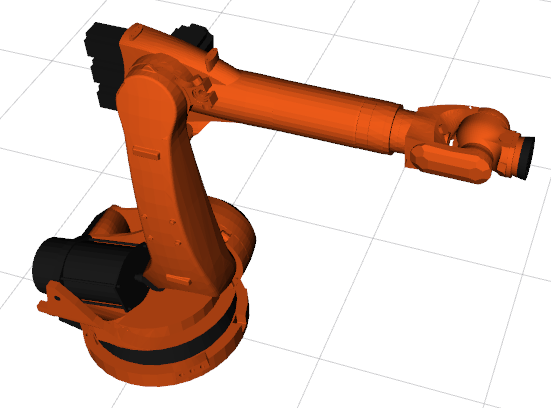
\includegraphics[width=0.7\linewidth]{kuka1}
	\caption[Rviz2 kuka]{Kuka KR210 in Rviz2.}
	\label{fig:kuka1}
\end{figure}
The robotic arm consists of six joints and seven links that connect them.
The six joints of the KR210 are numbered J1 to J6, and they allow the robot to move in various directions and orientations.
\begin{itemize}
	\item J1: The first joint is the base joint, which allows the robot to rotate horizontally around its vertical axis.
	
	\item J2: The second joint is the shoulder joint, which allows the robot to lift and lower its arm vertically.
	
	\item J3: The third joint is the elbow joint, which allows the robot to bend its arm vertically.
	
	\item J4: The fourth joint is the wrist roll joint, which allows the robot to rotate its wrist around its vertical axis.
	
	\item J5: The fifth joint is the wrist pitch joint, which allows the robot to tilt its wrist up and down.
	
	\item J6: The sixth joint is the wrist yaw joint, which allows the robot to rotate its wrist horizontally.	 
\end{itemize}

The arm also has links that connect the joints, including the base, lower arm, upper arm, wrist, and end-effector. These links are designed to provide strength and rigidity to the robot arm while allowing for smooth and precise movement. These links are:

\begin{itemize}
	\item Base Link: This is the fixed part of the robot that is attached to the ground.
	
	\item Link 1: This is the first link that connects the base to joint 1.
	
	\item Link 2: This link connects joint 1 to joint 2.
	
	\item Link 3: This link connects joint 2 to joint 3.
	
	\item Link 4: This link connects joint 3 to joint 4.
	
	\item Link 5: This link connects joint 4 to joint 5.
	
	\item End Effector (Link 6): This is the final link that connects to the tool or object being manipulated.
	
\end{itemize}


\begin{figure}[!tbp]
	\centering
	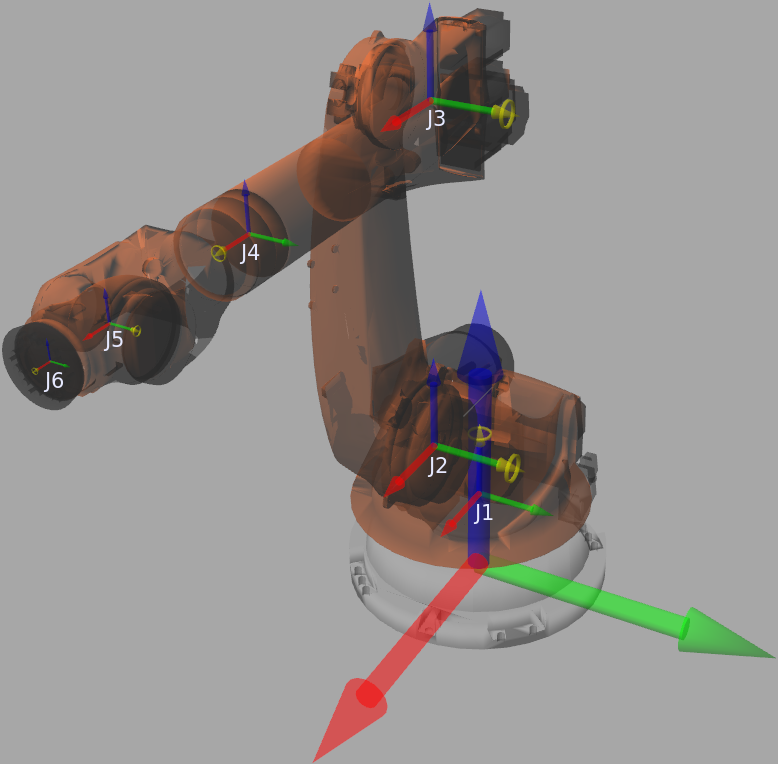
\includegraphics[width=0.9\linewidth]{kuka5}
	\caption[short caption]{long caption}
	\label{fig:kuka5}
\end{figure}

\begin{figure}[!tbp]
  \centering
  \subfloat[subcaption.]{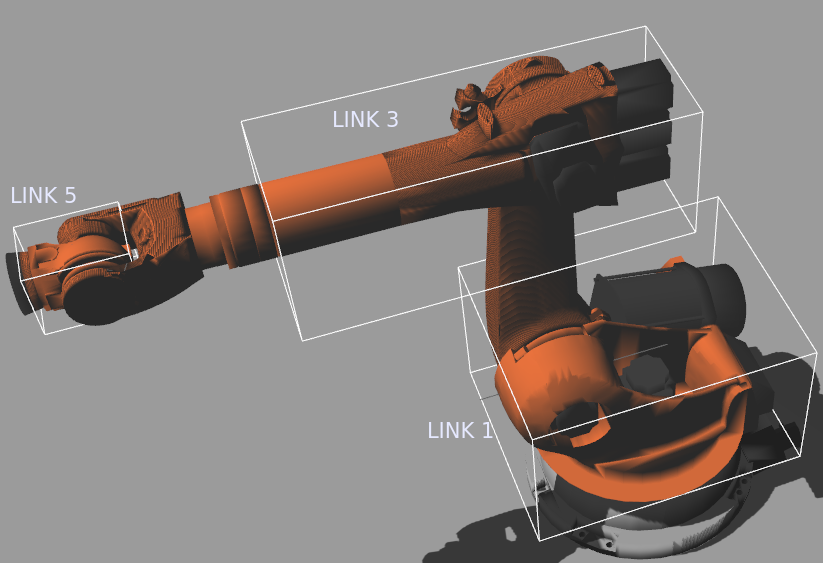
\includegraphics[width=0.45\textwidth]{kuka6}\label{fig:kuka6}}
  \hfill
  \subfloat[subcaption.]{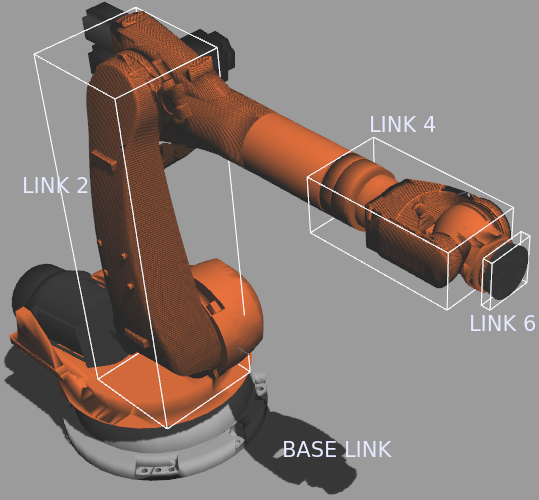
\includegraphics[width=0.45\textwidth]{kuka7}\label{fig:kuka7}}
  \caption{caption.}
\end{figure}




\begin{figure}[H]
	\centering
	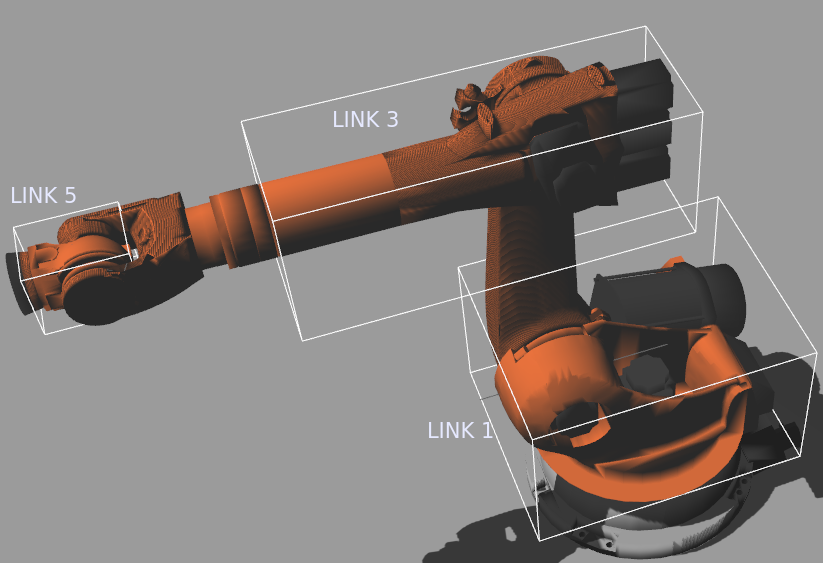
\includegraphics[width=0.7\linewidth]{kuka6}
	\caption[short caption]{long caption}
	\label{fig:kuka6o}
\end{figure}


A Bumper sensor was added to links 4, 5, and 6 to detect collisions with these links (As shown in the code snippet) to the URDF.

A Camera sensor is added (As shown in the code snippet) to the URDF.

The object the robotic arm has to learn to touch is a can taken from gazebo models (http://models.gazebosim.org/beer). A world file is created containing the can.

The Gazebo ROS state plugin was added (as shown in \ref{gazeboRosStatePluginXml}) to the world file to have the positions, velocities, and other properties from our models published and to be able to modify them programmatically.



\subsection{Moving the robotic arm}
The AnglesPublisher node was created to move the arm by publishing the target angles for the joints. To do this the Joint Trajectory Controller is used, this controller generates and executes trajectories for the robot joints. It subscribes to a JointTrajectory message that specifies the desired trajectory, and then generates a control signal to move the robot's joints along the trajectory. By publishing messages of type JointTrajectory to the joint\_trajectory topic the arm is moved.

\subsection{Getting Images from the camera}
The CameraSubscriber node was created to get images from the environment. The plugin previously used takes care of publishing the images to the topic /camera/image\_raw, the CameraSubscriber just subscribes to this topic and gets the images as messages of type Image.



ROS control module is used to move the arm. ROS Control is a framework for building and controlling robots in ROS (Robot Operating System). It provides a standardized way to manage hardware interfaces, controllers, and state machines, making it easier to develop and integrate robot applications.

The Joint State Broadcaster is a ROS node that broadcasts the state of robot joints. It reads joint positions, velocities, and efforts from a robot's hardware interfaces or controllers and publishes them as a JointState message on a ROS topic. This message contains the current state of all joints in the robot's model, allowing other ROS nodes to subscribe and use this information.

The Joint Trajectory Controller is a ROS controller that generates and executes trajectories for robot joints. It subscribes to a JointTrajectory message that specifies the desired trajectory, and then generates a control signal to move the robot's joints along the trajectory. It can use different algorithms to generate this control signal, such as PID, computed-torque, or model-predictive control. This controller is often used in combination with the Joint State Broadcaster to provide closed-loop control of the robot's joints.

Overall, the Joint State Broadcaster and Joint Trajectory Controller are two important components of ROS Control that enable the control of robot joints. The Joint State Broadcaster provides the current state of the joints to other ROS nodes, while the Joint Trajectory Controller generates and executes trajectories for the joints based on desired goals. Together, these components provide a powerful toolset for controlling robot motion in ROS. 



\begin{figure}[H]
	\centering
	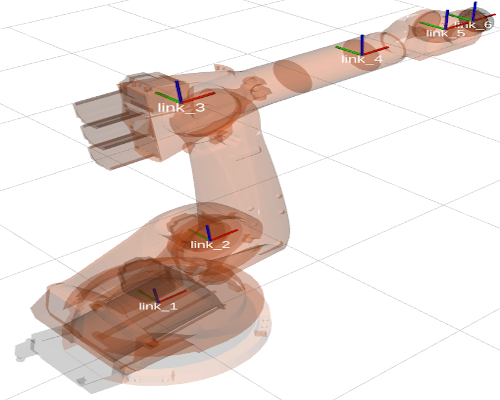
\includegraphics[width=0.5\linewidth]{kuka3}
	\caption[short caption]{long caption}
	\label{fig:kuka3}
\end{figure}

\begin{figure}[H]
	\centering
	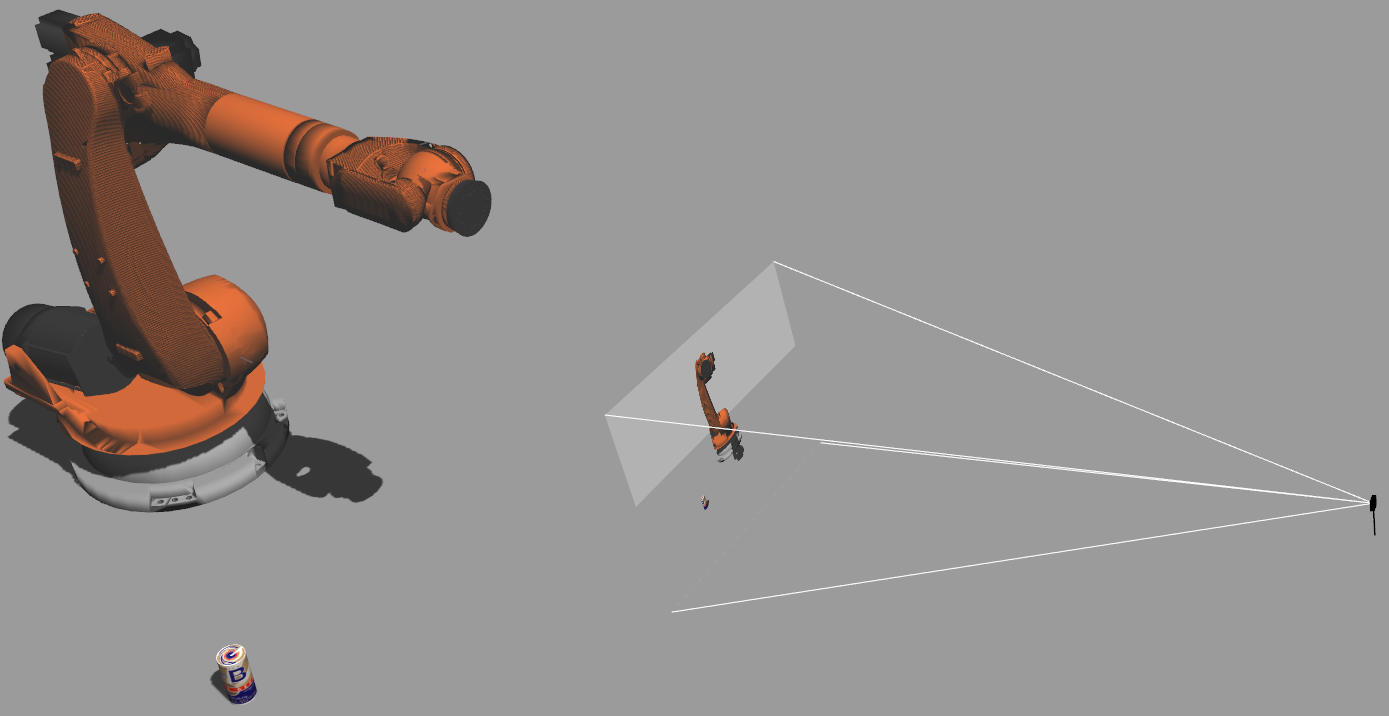
\includegraphics[width=0.95\linewidth]{kuka4}
	\caption[short caption]{long caption}
	\label{fig:kuka4}
\end{figure}



\begin{figure}[H]
\centering

\includegraphics[width=0.1\linewidth]{can}
\caption[short description]{long description}
\label{fig:can}
\end{figure}



Should refer, where possible, to the preceding chapter, e.e.:
Singular value decomposition of the matrix $\Sigma$ is conducted as explained in Sec.~\ref{sec:grundagen1} using the \textit{lapack} library (see Sec.~\ref{sec:grundlagen2}).

For software development: what is the logic of the developed code, which of it was done by yourself? Sequence diagrams or UML are good tools here.

Please give code snippets only if they take up less that 0.25 pages, and only if it is unavoidable. Longer snippets go to the appendix and are referenced like this: see App.~\ref{Snippet}.

\section{Experiments}\label{sec:exp}



\par\noindent\rule{\textwidth}{0.4pt}
Show here that the goals from the introduction were achieved (or not achieved), you need at least one experiment per goal. Use screenshots, diagrams, plots, photos, etc. as necessary.

\section{Discussion}
2-3 pages are a good idea here. Picks up goals from the introduction (see \ref{sec:ziele}) and experiments (see \ref{sec:exp}) and explains what was achieved and what was not (and why not in this case). Compares results with results from related work, see Sec.~\ref{sec:relwork}. Draws a preliminary conclusion for the whole thesis.

\section{Conclusion}
Give an executive summary for important decision makers here, as well as an outlook (what would you do if you had another 3 months). 2-3 pages are ok here.

\section{Using LaTeX, erase this chapter later}
%
I was too lazy to translate this, it will be translated later. But I believe the ideas are clear!
%
\subsection{Mathematische Gleichungen}
Eine mehrzeilige Gleichung sieht so aus (die Symbole nach den und-Zeichen werden untereinander gesetzt). Die nonmber-Befehle verhindern dass die Gleichung nummertiert wird (Geschmackssache, ist nie falsch wenn eine Gleichung nummeriert ist). Aber: eine Gleichung auf die man refernziert (also die ein Label hat), muss nummeriert sein!
\begin{align}
    A &= \sum_{i=1}^N x_i \label{eq:1}\nonumber\\
    B &= \frac{\pi}{2}
\end{align}

Eine inline-Gleichung: $x=45b + \frac{2}{3}\pi$. Der Text geht weiter! Auf inline-Gleichungen kann man keine Refernzen erstellen.

\subsection{Das ist eine Auflistung}
\begin{enumerate}
\item Element 1
\item Element 2
\end{enumerate}

\subsection{Das ist eine Bullet-Liste}
\begin{itemize}
\item Element 1
\item Element 2
\end{itemize}


\subsection{Eine Grafik bindet man so ein}
Zulässige Formate sind generell eps, pdf und png.
\begin{figure}[h]
    \centering
    
\includegraphics[width=0.8\textwidth]{logo.pdf}
    \caption{Logo der HAW Fulda}
    \label{fig:bildchen}
\end{figure}

\subsection{So schreibt man einen Algorithmus}

\begin{algorithm}[H]
 \KwData{this text}
 \KwResult{how to write algorithm }
 initialization\;
 \While{not at end of this document}{
  read current\;
  \eIf{understand}{
   go to next section\;
   current section becomes this one\;
   }{
   go back to the beginning of current section\;
  }
 }
 \caption{How to write algorithms\label{alg:dummy}
 }
\end{algorithm}

\subsection{So gestaltet man eine Tabelle}

\begin{table}[H]
\caption{Beispielstabelle\label{tab:beispiel}
}
\centering
\begin{tabular}{llr}
\hline
A    & B & C \\
\hline
D      & per gram    & 11.65      \\
          & each        & 1.01       \\
E       & stuffed     & 32.54      \\
F       & stuffed     & 73.23      \\
G & frozen      & 8.39       \\
\hline
\end{tabular}
\end{table}


\subsection{Interne Referenzen}
So wird ein Kapitel oder Unterkapitel referenziert: Kap.~\ref{sec:einleitung},
Kap.~\ref{sec:webquellen}. Auf Gleichungen bezieht man sich so: Wie in Gl.~(\ref{eq:1}) gezeigt,
sehen Gleichungen in der Regel gut aus. Auf Abb.~\ref{fig:bildchen} bezieht man sich so. Auf
Tab.~\ref{tab:beispiel} referenziert man so. Algorithmen sind analog: siehe Alg.~\ref{alg:dummy}.
Generell kann man alles zitieren was ein Label hat.

\subsection{Textformatierung}
\textbf{So wird dick geschrieben} und \textit{so kursiv}.

\subsection{Zitieren}\label{sec:zitate}
Generell zitiert man so: wie in \cite{clemen1989combining} gezeigt, blablaba. Für jedes zitierte Werk ist ein BibTex-Eintrag nötig! Eine gute Quelle ist Google Scholar!!

\subsection{Webquellen zitieren}\label{sec:webquellen}
So wird eine Webquelle zitiert: \cite{shiny1}, siehe auch den Eintag im BibTeX-File.
Wichtig: für jede Web-Quelle ein BibTeX-Eintrag! Wenn Sie das auf die hier gezeigte Art machen, werden URLs (fast) automatisch getrennt. Kontrollieren Sie trotztdem die Literaturliste, es kann sein dass das nicht immer funktioniert.

\subsection{Literaturverzichnis erstellen}
Hierzu müssen BibTeX-Einträge in die Datei literatur.bib eingefügt werden. Die BibTeX-Keys sind jeweils Argumente für die cite-Kommandos! Wenn Sie literatur.bib ändern müssen Sie alles mindestens 5x compilieren: 3x mit latex, 1x mit BibTex und dann noch 2x mit LaTeX (in der Reihengfolge). Am besten Sie machen ein Skript dafür!

%\subsection{Erstellung eines PDFs im PDF-A Format}
%Durch Einbinden geeigneter Packages (pdfx) wird diese Vorlage bereits als PDF-A erzeugt. Sie sollten allerdings die Metadaten in der Datei main.xmpdata anpassen!

%%%%%%%%%%%%%%%%%%%%%%%%%%%%
%% Literaturverzeichnis wird
%% automatisch eingefügt
%%%%%%%%%%%%%%%%%%%%%%%%%%%%
\clearpage
\bibliographystyle{unsrt}
\bibliography{literatur}

%\lhead{}
%\printbibliography
%\addcontentsline{toc}{section}{\bibname}
\appendix
\section{Code Snippets}
\begin{listing}[htbp]
\begin{minted}[fontsize=\footnotesize,linenos=false,escapeinside=||,samepage]{xml} 
  <gazebo reference="link_4">
    <!-- contact sensor -->
    <sensor name="end_effector_sensor" type="contact">
      <selfCollide>true</selfCollide>
      <alwaysOn>true</alwaysOn>
      <update_rate>500</update_rate>
      <contact>
        <collision>link_4_collision</collision>
      </contact>
      <!-- gazebo plugin -->
      <plugin name="gazebo_ros_bumper_sensor" filename="libgazebo_ros_bumper.so">
        <ros>
          <namespace>contact_sensor</namespace>
          <remapping>bumper_states:=bumper_link_4</remapping>
        </ros>
        <frame_name>link_4</frame_name>
      </plugin>
    </sensor>
  </gazebo>
\end{minted}
\caption{Bumper Sensor}
\label{bumperSensorXml}
\end{listing}

\begin{listing}[htbp]
\begin{minted}[fontsize=\footnotesize,linenos=false,escapeinside=||,samepage]{xml} 
  <gazebo reference="camera_link">
    <material>Gazebo/Black</material>
    <sensor name="camera" type="camera">
      <pose>0 0 0 0 0 0</pose>
      <visualize>true</visualize>
      <update_rate>10</update_rate>
      <camera>
        <horizontal_fov>1.089</horizontal_fov>
        <image>
          <format>R8G8B8</format>
          <width>640</width>
          <height>480</height>
        </image>
        <clip>
          <near>0.05</near>
          <far>8.0</far>
        </clip>
      </camera>
      <plugin name="camera_controller" filename="libgazebo_ros_camera.so">
        <frame_name>camera_link_optical</frame_name>
      </plugin>
    </sensor>
  </gazebo>
\end{minted}
\caption{Camera Sensor}
\label{cameraSensorXml}
\end{listing}

\begin{listing}[htbp]
\begin{minted}[fontsize=\footnotesize,linenos=false,escapeinside=||,samepage]{xml} 
<plugin name='gazebo_ros_state' filename='libgazebo_ros_state.so'>
  <ros>
    <namespace>/gazebo_state</namespace>
    <argument>model_states:=model_states_demo</argument>
    <argument>link_states:=link_states_demo</argument>
  </ros>
  <update_rate>1.0</update_rate>
</plugin>
\end{minted}
\caption{Gazebo ROS state plugin}
\label{gazeboRosStatePluginXml}
\end{listing}

\begin{listing}[htbp]
\begin{minted}[fontsize=\footnotesize,linenos=false,escapeinside=||,samepage]{xml} 
  <gazebo>
    <plugin filename="libgazebo_ros2_control.so" name="gazebo_ros2_control">
      <robot_sim_type>gazebo_ros2_control/GazeboSystem</robot_sim_type>
      <parameters>/home/ros/ros2-projects/my-workspace/src/kuka_kr210/config/jtc.yaml</parameters>
    </plugin>
  </gazebo>
\end{minted}
\caption{Gazebo plugin and ROS2 controller configuration file.}
\label{gazeboPluginControllerConfigFile}
\end{listing}

\begin{mdframed}[linecolor=black, topline=false, bottomline=false,leftline=false, rightline=false, backgroundcolor=white]
\begin{minted}[fontsize=\small,linenos=false,escapeinside=||,]{xml} 
  <ros2_control name="GazeboSystem" type="system">
    <hardware>
      <plugin>gazebo_ros2_control/GazeboSystem</plugin>
    </hardware>
    <joint name="joint_1">
      <command_interface name="position">
        <param name="min">-3.14</param>
        <param name="max">3.14</param>
      </command_interface>
      <command_interface name="velocity">
        <param name="min">-3.15</param>
        <param name="max">3.15</param>
      </command_interface>
      <state_interface name="position"/>
      <state_interface name="velocity"/>
      <state_interface name="effort"/>
      <param name="initial_position">0.0</param>
    </joint>
    <joint name="joint_2">
      <command_interface name="position">
        <param name="min">-3.14</param>
        <param name="max">3.14</param>
      </command_interface>
      <command_interface name="velocity">
        <param name="min">-3.15</param>
        <param name="max">3.15</param>
      </command_interface>
      <state_interface name="position"/>
      <state_interface name="velocity"/>
      <state_interface name="effort"/>
      <param name="initial_position">-1.57</param>
    </joint>
    <joint name="joint_3">
      <command_interface name="position">
        <param name="min">-3.14</param>
        <param name="max">3.14</param>
      </command_interface>
      <command_interface name="velocity">
        <param name="min">-3.15</param>
        <param name="max">3.15</param>
      </command_interface>
      <state_interface name="position"/>
      <state_interface name="velocity"/>
      <state_interface name="effort"/>
      <param name="initial_position">0.0</param>
    </joint>
    <joint name="joint_4">
      <command_interface name="position">
        <param name="min">-3.14</param>
        <param name="max">3.14</param>
      </command_interface>
      <command_interface name="velocity">
        <param name="min">-3.2</param>
        <param name="max">3.2</param>
      </command_interface>
      <state_interface name="position"/>
      <state_interface name="velocity"/>
      <state_interface name="effort"/>
      <param name="initial_position">-1.57</param>
    </joint>
    <joint name="joint_5">
      <command_interface name="position">
        <param name="min">-3.14</param>
        <param name="max">3.14</param>
      </command_interface>
      <command_interface name="velocity">
        <param name="min">-3.2</param>
        <param name="max">3.2</param>
      </command_interface>
      <state_interface name="position"/>
      <state_interface name="velocity"/>
      <state_interface name="effort"/>
      <param name="initial_position">0.0</param>
    </joint>
    <joint name="joint_6">
      <command_interface name="position">
        <param name="min">-3.14</param>
        <param name="max">3.14</param>
      </command_interface>
      <command_interface name="velocity">
        <param name="min">-3.2</param>
        <param name="max">3.2</param>
      </command_interface>
      <state_interface name="position"/>
      <state_interface name="velocity"/>
      <state_interface name="effort"/>
      <param name="initial_position">0.0</param>
    </joint>
  </ros2_control>
\end{minted}
\end{mdframed}

%\begin{figure}
%    \centering
%    %\includegraphics{s}
%    \caption{Normalerweise bindet man Snippets als Bilder ein...\label{Snippet}
%    }
%\end{figure}

\section{Thesis defence}
The defence is 15/20 minutes for Bachelor/Master, followed by questions and a discussion. Both examiners are present, and you can invite external persons since defences are generally public.

Targetted group are non-computer scientists, e.g., from higher management, NOT the examiners. Means that at least $\frac 1 3$ if the presentation is introduction/context/problem statement. You should re-use text/images/graphs/etc from the corresponding chapters here!

1 Slide per minute is a good guideline. If you can guess that some questions are going to be asked anyway, prepare some slides specifically for these questions, makes a good impression, and you can show them in the discussion time, not during the 15 minutes of the presentation.

Defences are not graded, you can only pass or not pass. 

Students are responsible for finding dates for the defence and coordinating this with both supervisors. 

Some common advice is:
\begin{itemize}
    \item Speak slowly and loadly
    \item If you do not have enough time left for all slides, leave some out rather than rushing through all of them!!
    \item Slide numbers!
    \item In presence: be there 10 minutes ahead of time to check projectors etc. Makes a very bad impression if this is not working. Same for online presentations: be there 5 minutes ahead of time to verify screen sharing works.
    \item do not read text from the slides. These should contains key words only, and you explain the rest in free presentation
    \item Defences can by all means be online, more convenient for companies
    \item in presence: always carry a USB key with a PDF of your slides. If you have to use another PC than yours, PowerPoint slides may look very differently (fonts, page setup etc.)
    \item No-Go: spelling errors on slides!!!
    \item Do not use animations, they may not work in an online setting
\end{itemize}

%%%%%%%%%%%%%%%%%%%%%%%%%%%%
%% Eidesstattliche Erklärung
%% muss angepasst werden
%% in Erklaerung.tex
%%%%%%%%%%%%%%%%%%%%%%%%%%%%
%\newpage
%\begin{otherlanguage}{ngerman}
%\thispagestyle{empty}
%\section*{Eidesstattliche Erklärung}
%\thispagestyle{empty}
%Hiermit versichere ich, die vorliegende Arbeit selbstständig verfasst und keine anderen als die angegebenen Quellen und Hilfsmittel benutzt sowie die Zitate deutlich kenntlich gemacht zu haben.
%\newline
%Ich erkläre weiterhin, dass die vorliegende Arbeit in gleicher oder ähnlicher Form noch nicht im Rahmen eines
%anderen Prüfungsverfahrens eingereicht wurde.
%\vspace{4\baselineskip}\\
%Würzburg, den \today \hfill Autor
%\vspace{4\baselineskip}\\
%\end{otherlanguage}


\section{Extras}
\subsection{Markov Decision Process}
A Markov Decision Process (MDP) is defined by a tuple $<S, A, P, R, \gamma>$, where:

\begin{itemize}
\item $S$ is the set of states in the environment
\item $A$ is the set of actions that can be taken in each state
\item $P$ is the state transition probability matrix, where $P_{ss'}^a = \mathbb{P}[S_{t+1} = s' \mid S_t = s, A_t = a]$
\item $R$ is the reward function, where $R_s^a = \mathbb{E}[R_{t+1} \mid S_t = s, A_t = a]$
\item $\gamma$ is the discount factor, where $\gamma \in [0, 1]$
\end{itemize}

The goal of an agent in a Markov Decision Process is to find a policy $\pi: S \rightarrow A$ that maximizes the expected discounted reward:

\begin{equation*}
V_\pi(s) = \mathbb{E}\pi\Bigg[\sum{k=0}^\infty \gamma^k R_{t+k+1} \Bigg| S_t = s\Bigg]
\end{equation*}

or the corresponding action-value function:

\begin{equation*}
Q_\pi(s, a) = \mathbb{E}\pi\Bigg[\sum{k=0}^\infty \gamma^k R_{t+k+1} \Bigg| S_t = s, A_t = a\Bigg]
\end{equation*}

\subsection{Q learning Algorithm}
The Q-learning algorithm is an off-policy temporal difference learning algorithm for finding the optimal action-value function $Q^(s, a)$ in a Markov Decision Process (MDP). The algorithm updates an estimate of $Q^(s, a)$ by iteratively applying the following update rule:

\begin{equation*}
Q(s_t, a_t) \leftarrow Q(s_t, a_t) + \alpha\Big[ R_{t+1} + \gamma\max_{a} Q(s_{t+1}, a) - Q(s_t, a_t) \Big]
\end{equation*}

where $s_t$ and $a_t$ are the current state and action, $R_{t+1}$ is the reward received after taking action $a_t$ in state $s_t$ and transitioning to state $s_{t+1}$, $\alpha$ is the learning rate, and $\gamma$ is the discount factor.

The Q-learning algorithm can be summarized as follows:

\begin{enumerate}
\item Initialize the Q-value function $Q(s, a)$ for all state-action pairs.
\item Observe the current state $s_t$.
\item Choose an action $a_t$ based on a policy, such as $\epsilon$-greedy or softmax.
\item Take the action $a_t$ and observe the next state $s_{t+1}$ and reward $R_{t+1}$.
\item Update the Q-value function using the update rule: $Q(s_t, a_t) \leftarrow Q(s_t, a_t) + \alpha\Big[ R_{t+1} + \gamma\max_{a} Q(s_{t+1}, a) - Q(s_t, a_t) \Big]$.
\item Set $s_t = s_{t+1}$ and repeat from step 3 until the end of the episode or termination of the task.
\end{enumerate}

The Q-learning algorithm is guaranteed to converge to the optimal action-value function $Q^*(s, a)$ under certain conditions, such as the MDP being finite and the learning rate $\alpha$ decaying over time.

\subsection{Deep Q Learning}
Deep Q-learning is a variant of the Q-learning algorithm that uses a deep neural network to approximate the action-value function $Q(s, a)$ in a Markov Decision Process (MDP). The algorithm combines reinforcement learning with deep neural networks to enable learning in high-dimensional and continuous state spaces.

The Deep Q-learning algorithm can be summarized as follows:

\textbf{Algorithm: Deep Q-learning}

\begin{enumerate}
\item Initialize the replay memory buffer $D$ with capacity $N$.
\item Initialize the Q-network with random weights $\theta$.
\item Initialize the target Q-network with weights $\theta^{-} = \theta$.
\item For each episode $e=1,2,...,E$ do the following:
\begin{enumerate}
\item Initialize the environment with initial state $s_0$.
\item For each step $t=1,2,...,T$ do the following:
\begin{enumerate}
\item With probability $\epsilon$ select a random action $a_t$, otherwise select $a_t=\arg\max_{a} Q(s_t, a; \theta)$.
\item Execute action $a_t$ and observe reward $r_t$ and next state $s_{t+1}$.
\item Store the transition $(s_t, a_t, r_t, s_{t+1})$ in the replay memory buffer $D$.
\item Sample a mini-batch of transitions $(s_j, a_j, r_j, s_{j+1})$ from the replay memory buffer $D$.

\item Compute the Q-learning target for each transition $(s_j, a_j, r_j, s_{j+1})$:

 $y_j = \begin{cases} r_j & \text{if episode terminates at step } j+1 \\ r_j + \gamma\max_{a'}Q(s_{j+1},a';\theta^{-}) & \text{otherwise} \end{cases}$.

\item Compute the loss between the predicted Q-value and the target Q-value: $L(\theta) = \frac{1}{B}\sum_{j=1}^B(y_j-Q(s_j,a_j;\theta))^2$.
\item Update the Q-network weights using stochastic gradient descent: $\theta \leftarrow \theta - \alpha\nabla_\theta L(\theta)$.
\item Every $C$ steps update the target Q-network weights: $\theta^{-} \leftarrow \tau\theta + (1-\tau)\theta^{-}$.
\item Set $s_t=s_{t+1}$.
\end{enumerate}
\end{enumerate}
\end{enumerate}

In the Deep Q-learning algorithm, the replay memory buffer $D$ is used to store experiences in order to prevent overfitting and stabilize learning. The target Q-network is used to compute the target Q-value in the Q-learning update, and its weights are periodically updated from the Q-network to prevent target overestimation.

The Deep Q-learning algorithm has been successfully applied to various tasks, such as playing Atari games, controlling robots, and playing board games.




The Deep Q-learning algorithm uses experience replay and target networks to improve stability and convergence of the algorithm. Experience replay randomly samples transitions from the replay memory buffer to decorrelate the data and prevent overfitting. Target networks are used to stabilize the training by keeping a separate target network with fixed parameters and periodically updating it with the weights of the online network.

The Deep Q-learning algorithm has been successfully applied to various tasks, such as playing Atari games, controlling robots, and playing board games.








\end{document}

